
In this section we describe the adaptations that have been made to the reference implementation of TLSF to make it more suited toward being used in the context of a garbage collector, specifically ZGC.

\subsection{Architectural Considerations}

ZGC is solely implemented for 64-bit architecture and does not support 32-bit~\cite{zgc_deep_dive}. Hence, in our effort to adapt the allocator for ZGC, it is reasonable for the allocator to also be limited to the same scope. The authors of TLSF have designed their allocator primarily for 32-bit systems due to it being targeted toward real-time embedded systems, which usually operate on 32-bit architecture. However, while TLSF was initially designed with 32-bit systems in mind, its design principles and concepts are not inherently tied to any specific architecture. Hence, adapting the allocator to 64-bit systems does not require any significant changes in its design, apart from aligning memory toward the allocation unit of 8 bytes for 64-bit systems instead of 4 bytes for 32-bit systems.

\subsection{General and Optimized Versions}

When adapting the allocator we will consider the use cases of either using it as a normal allocator in cases where a traditional malloc/free combination is used, or as a way to allocate objects on pages in ZGC. To minimize the codebase, which is desirable from a maintenance perspective, the allocator will be adapted in a way which allows it to be configured for different use-case. A major benefit of doing this is that different configurations can easily be compared against each other, streamlining the process of measuring efficacy of any adaptations that are made.

Worth noting however, is that in the process of redesigning the allocator in a configurable manner, some changes that deviates from the reference implementation will have to be made. Such trade-offs, which will be discussed in more detail later, could be reasonable when extending the interface for supporting multiple configurations, or versions, of the allocator.

\subsection{Reduced Allocation Size Range}

In ZGC, small and medium pages only allow the user to allocate in certain size ranges. To our advantage, we can use this to store metadata about the allocator in a more efficient way. Small pages allow sizes in the range [16B, 256KB] and medium pages (256KB, 4MB]. We note that the allowed sizes in the medium range is a factor of 16KB larger than the small range. This allows us to limit the allocator to the size range of small page, with an additional multiplication factor of 1 for small pages and 16KB for medium pages.

With the limited allocation size range for small pages in mind, we are able to limit the number of free-lists we need and in turn the bits used in the bitmaps. We need 14 first-levels to be able to index every power of two inside the small page range, with a lower-bound of $2^4 =$ 16B and an upper-bound of $2^{17} =$ 128KB. It is desirable to store all bitmap information in a single 64-bit word for performance reasons, both in terms of cache efficiency and usage of efficient bit instructions. If we want to stay inside the 64-bit limit, we must choose the number of second-levels accordingly. For efficiency reasons again, the number of second levels should be a power of two~\cite{TLSF} so that bit-shift instructions can be used. The only value this leaves us is 4, which requires $14 * 4 =$ 56 bits for storing all metadata.

Since a page is initially 2MB large, the initial block will be significantly larger than the maximum allocation size of 256KB. This means we either need to split it up into multiple blocks of smaller sizes or store it in a different free-list. To solve this we will add a last free-list that is called the "large-list", represented by the 57th bit. The large-list will store blocks that are above the largest index to support storing blocks that are initially very large.

Combining the insight of the number of required first- and second-levels, desire to use a single 64-bit bitmap and large-list, we can construct a new bitmap representation, as shown in Figure~\ref{fig:bitmap_flattening}. The new bitmap disregards the literal notion of ``Two Level'' from Two Level Segregated Fit and flattens the first- and second-level bitmaps to a single bitmap. The new bitmap is indexed using the formula: 
\[
    \text{bitmap\_index($f, s$)} = f * 4 + s
\]
where $f$ and $s$ are the first- and second-level indexes respectively. Additionally, the lowest size classes have been placed at the least significant bits of the bitmap to make searching for the next non-empty free-list efficient using the find-first-set bit instruction.

\begin{figure}[H]
    \centering
    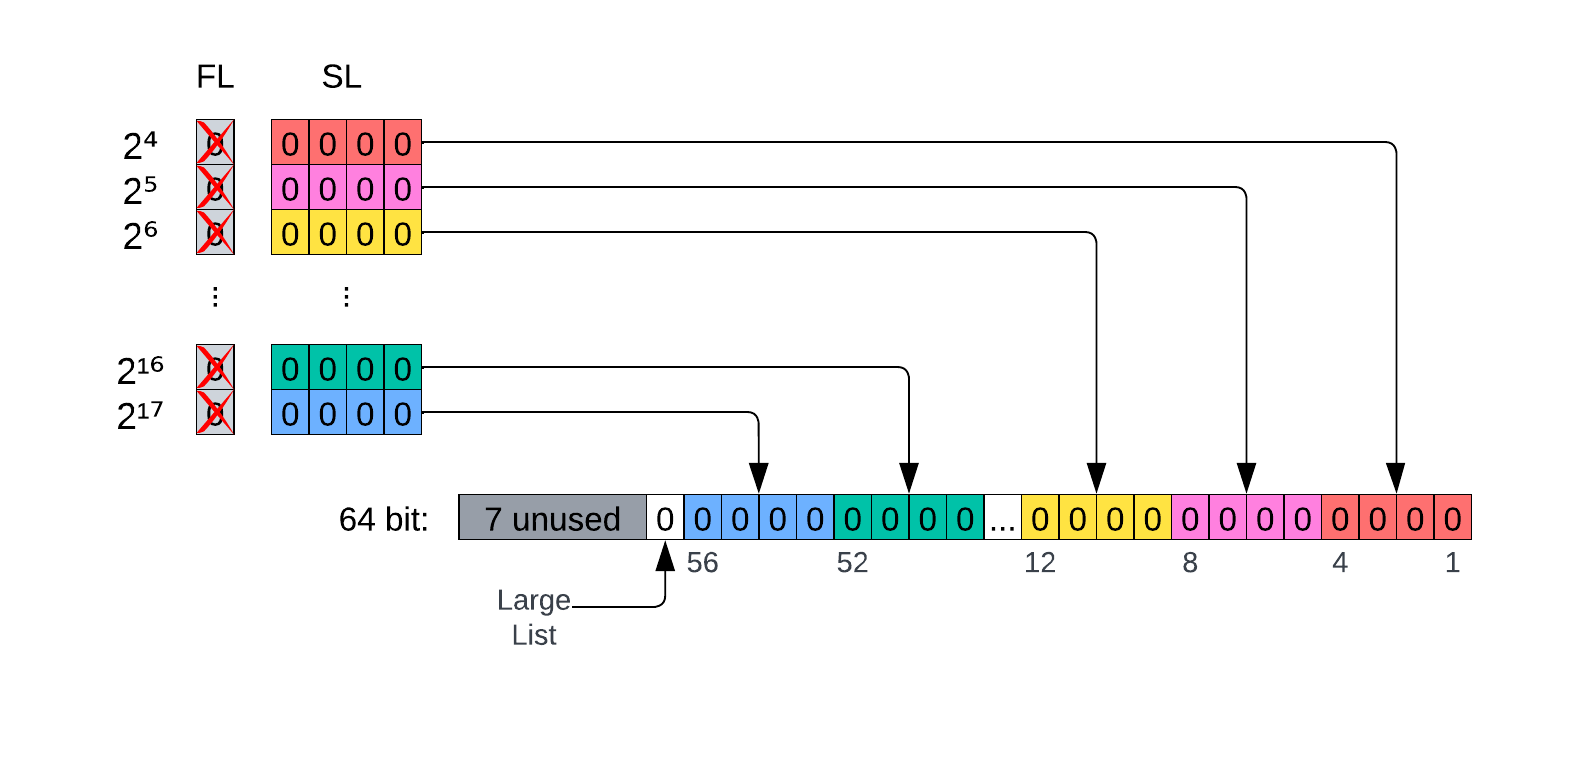
\includegraphics[width=1\textwidth]{figures/bitmap_flattening.png}
    \caption{Flattening of the 2D-matrix representation of TLSF bitmaps into a single 64-bit value. The first-level bitmap is disregarded in favor of indexing the new flattened bitmap using the first-level value instead. The number of first-levels are 14, indicated by bits of the same color belonging to the same first-level. The number of second-levels are 4, as indicated by the same number of colored bits.}
    \label{fig:bitmap_flattening}
\end{figure}

The correlation between the bitmap and the free-lists is depicted in Figure~\ref{fig:bitmap_relationship}, adhering closely to the original TLSF design. However, the adaptation now efficiently determines the relevant free-list by looking in the single bitmap, not two bitmaps as in the original design.

\begin{figure}[H]
    \centering
    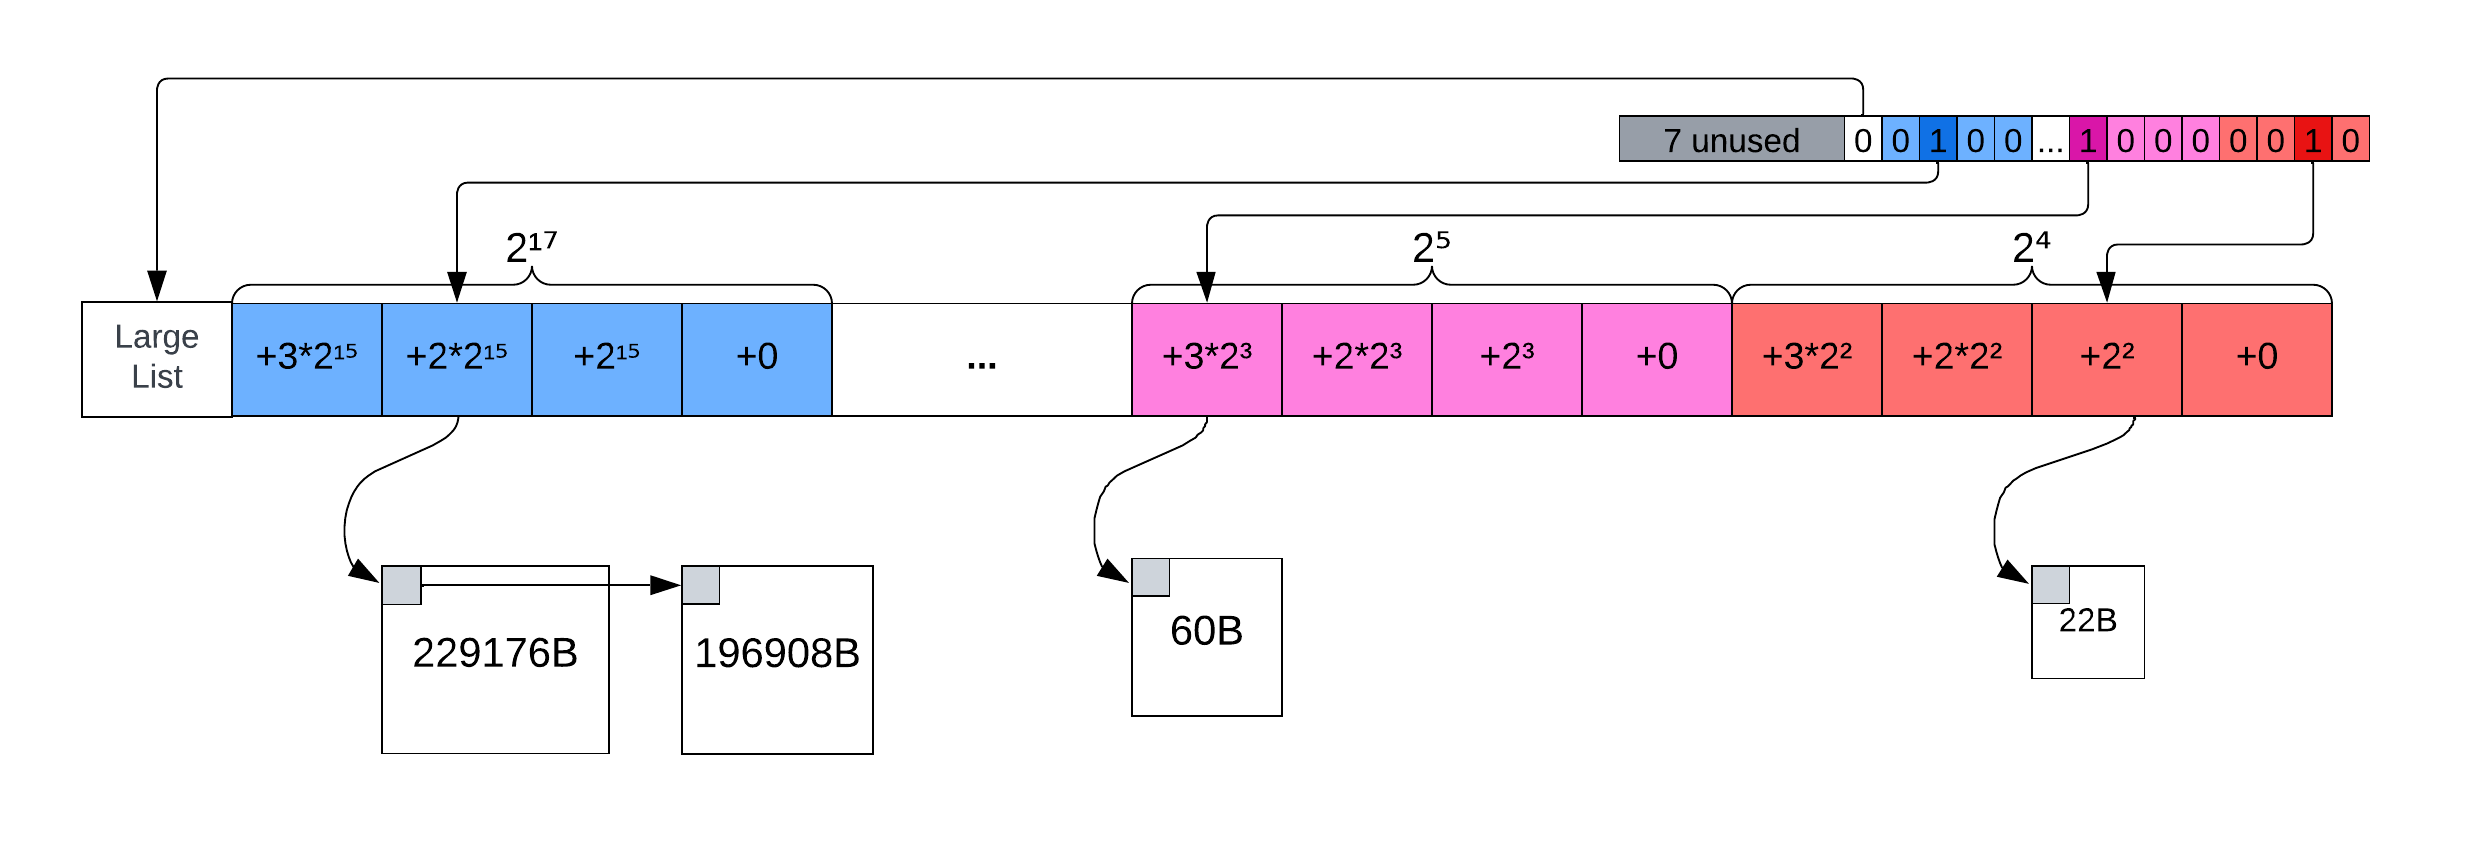
\includegraphics[width=1\textwidth]{figures/bitmap_relationship.png}
    \caption{Relationship between the new bitmap representation and accessing the corresponding free-lists.}
    \label{fig:bitmap_relationship}
\end{figure}

% TODO: Detta borde flyttas till discussion.
% A drawback of dividing the memory into only four second-levels per fist-level is that there is less chance that a block is closer to the size that we want to allocate. This could potentially lead to higher fragmentation, as there are fewer size classes of blocks available. However, this is generally not a problem...

% TODO: Cite TLSF paper.
% Benefits: Reduced memory overhead, cache efficiency, Simplified indexing (and Atomic operations??)
% Drawbacks: Reduce number of second-level partitions to 4, instead of more, which could have an impact on internal fragmentation.

\subsection{Transitioning Between Different Allocation Strategies}

Completely phasing out the utilization of bump-pointer allocation may not be optimal, especially when there is no constant requirement to allocate solely within the ``holes'' of a page. Instead, users could employ bump-pointer allocation up to a certain point, at which it becomes advantageous to transition to a more sophisticated allocator for non-bump-pointer allocation.

Most allocators start with an unused chunk of memory, allowing them to track and keep an up-to-date record of what the underlying memory contains. However, in the case where transitioning from bump-pointer to using an allocator, the underlying memory have contents that is not represented in the allocator. To solve this, we need to update the allocator's internal representation to align with the contents of the memory. In ZGC, the latest live analysis of a page contains an accurate representation of what data is alive in the page's underlying memory. This information can therefore be used to update the allocator's internal representation after a transition to using an allocator.

The construction of the allocator's representation involves a two-step process that extends the optimized allocator's API. Initially, the representation must be cleared so that any previous data is removed. When clearing the allocator, a block is allocated to cover the entirety of the underlying memory. This allows the user to invoke a function to free blocks within specified ranges, allowing to selectively ``carve'' segments free memory from the initially allocated block. When freeing ranges of memory, we only consider four cases: 

\begin{enumerate}
    \item The range is strictly within an allocated block and does not start nor end on the block's edges.
    \item The range begins at the start of the block and ends on the end of the block.
    \item The range starts inside the block and ends on the block's end.
    \item The range starts at the block's start and ends inside the block.
\end{enumerate}

We will not consider cases where the range overlaps multiple blocks and start or end on the edge of a block that is not the last or the first block in the physical order. This is because if a user wants to free a consecutive range of 64 bytes for example, they should always free the entire 64 byte range directly and not the first 32 bytes followed by the next 32 bytes. This reduces complexity of the implementation without significantly impacting user functionality.

\subsection{Deferred Coalescing of Blocks}

In the process of allocating and freeing blocks within an allocator, the general preference is to always have as large blocks as possible available to fulfill larger requests. However, in scenarios where numerous small allocations are frequently made and free'd, the emphasis on coalescing blocks to accommodate larger requests in the future may not be worthwhile. Instead, coalescing of blocks will be deferred until a later point in time or none at all.

The idea behind deferred coalescing is that when the user calls free(), the block being freed is not implicitly attempted to be coalesced with its adjacent physical neighbors. Instead, the allocator's API is extended to include an explicit coalesce operation. This operation scans through all blocks and coalesces as many as possible. Unlike immediate coalescing, this deferred approach postpones the process until a later point when a larger block is required.

The explicit coalesce operation conducts a pass over all blocks, requiring only knowledge of the size of the current block to identify the location of the next block. This eliminates the need to store a pointer to the physical neighbor right before the current block, which is only used when coalescing in a free() call. The algorithm describing how the pass is done is shown in Algorithm~\ref{algorithm:coalesce_blocks}.

\begin{algorithm}[H]
current = first\_physical\_block\\
\While{current != nullptr} {
next = get\_next\_block(current)\;
\uIf{next != nullptr \textbf{and} current->is\_free() \textbf{and} next->is\_free()} {
    current = coalesce\_neighbors(current, next)\;
    insert\_block(current)\;
}
\Else {
    current = next
}
}
\label{algorithm:coalesce_blocks}
\caption{Algorithm for explicitly coalescing all possible free blocks in the allocator. Note that coalesce\_neighbors() removes both blocks from the free-list before the newly coalesced block is inserted.}
\end{algorithm}

\subsubsection{Disregarding Size for Allocated Blocks}

\subsubsection{Block Header Adjustments}

R. Jones et al~\cite[Page 103]{gchandbook} discuss that in the context of using allocators in garbage collectors, it is a reasonable approach to remove certain parts of the so called boundary tag, or block header for TLSF. This is because a garbage collector know significantly more about the memory being processed than what a traditional system using a general purpose memory allocator does. This allows us to, for example, defer coalescing by default, transition between different allocators and optimize the bitmap layout from knowing what sizes will be allocated beforehand.

Combining the insights from the adaptations made so far, we can observe that storing a pointer to the previous physical block is no longer needed in the optimized version. This is because the previous physical pointer is only used when calling free and coalescing blocks with their physical neighbors. Following this, we will redesign the header for the previous physical pointer to be removed in the optimized version and still kept in the general version. 

% TODO: Disadventageous for small allocations, will have to be measured in practice.

The block header, as used in the reference implementation, is shown in Figure~\ref{fig:blockheader_adap_reference}. Here, the next and prev pointers are stored in the unused parts of free blocks and are unused in allocated blocks. In contrast, Figure~\ref{fig:blockheader_adap_general} shows the adapted block header for the general version of the allocator. In this version, all four fields are used for both free and allocated blocks since the previous physical pointer has been rearranged to the end of the header. Rearranging the previous physical pointer allows us to get the block header for optimized blocks, as shown in Figure~\ref{fig:blockheader_adap_optimized}. In the optimized header, the next and prev pointers have been converted to offsets, allowing them to be 32-bits each. Additionally, both the size and the now next/prev offsets are only stored in the unused parts of free blocks, allowing for a 0-byte header for allocated blocks.

% In the optimized header, the only constant overhead is the size field, as the next and prev pointers are only used in the unused parts of free blocks, as in the reference implementation. Additionally, the previous physical pointer is completely ignored in the optimized header.

\begin{figure}[H]
    \centering
    \begin{subfigure}[b]{0.3\textwidth}
        \centering
        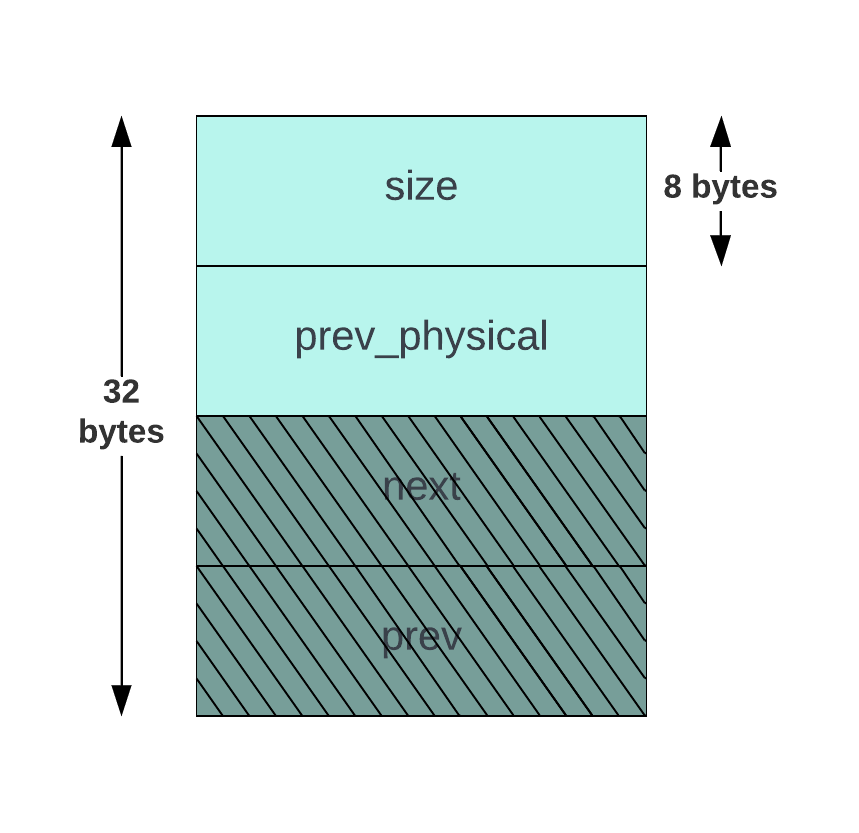
\includegraphics[width=\textwidth]{figures/blockheader_adap_reference.png}
        \caption{Reference implementation block header.}
        \label{fig:blockheader_adap_reference}
    \end{subfigure}%
    \hfill
    \begin{subfigure}[b]{0.3\textwidth}
        \centering
        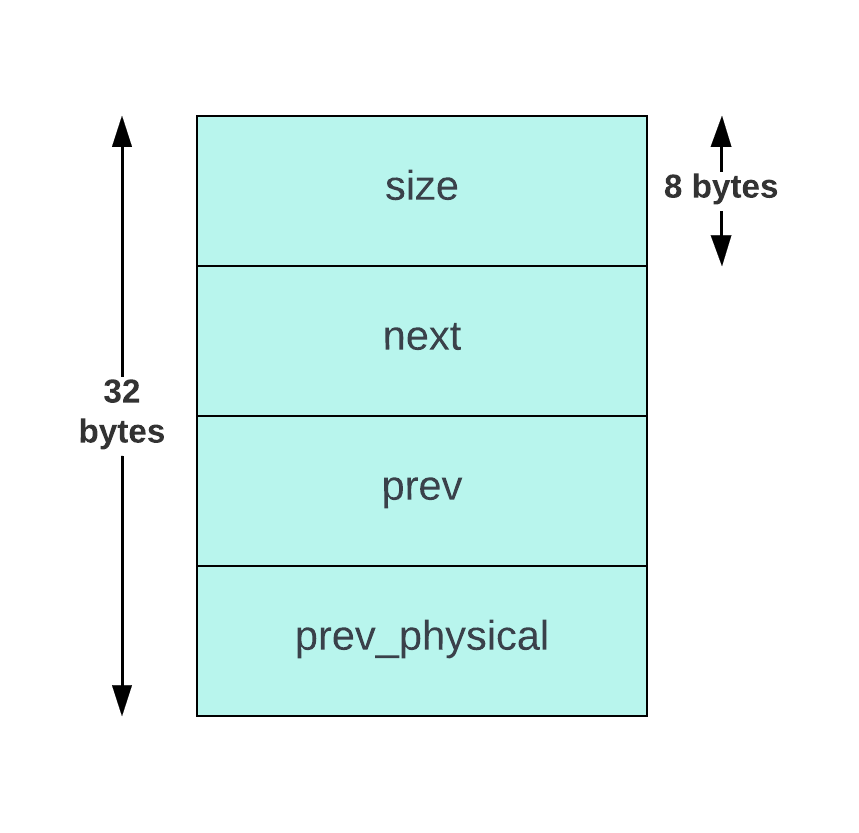
\includegraphics[width=\textwidth]{figures/blockheader_adap_general.png}
        \caption{Adapted general block header.}
        \label{fig:blockheader_adap_general}
    \end{subfigure}%
    \hfill
    \begin{subfigure}[b]{0.3\textwidth}
        \centering
        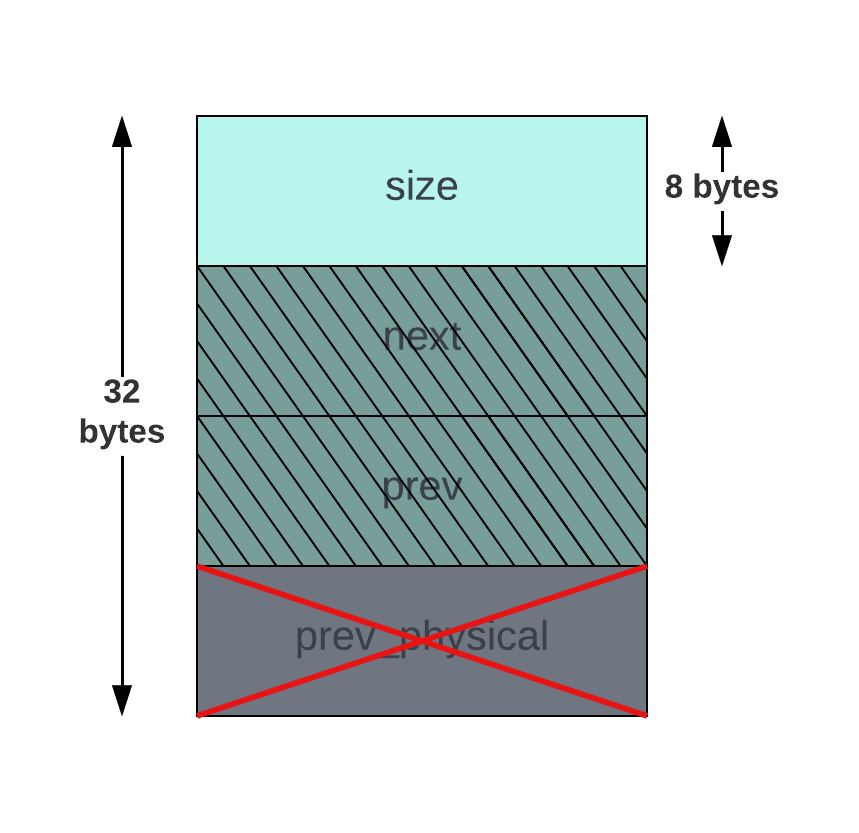
\includegraphics[width=\textwidth]{figures/blockheader_adap_optimized.png}
        \caption{Adapted optimized block header.}
        \label{fig:blockheader_adap_optimized}
    \end{subfigure}
    \caption{Overview of block header contents and adaptations. Dashed fields are only unused in the unused part of free blocks and crossed out fields are unused.}
    \label{fig:blockheader_adaptations}
\end{figure}

The goal of changing the header is to reduce the constant block header overhead required when allocating blocks. This is especially important when most allocations are small, where the block overhead is most significant. With the new design for the block header, the constant block header overhead for the optimized version is reduced to only 8 bytes for storing the size of the block. However, reducing the overhead for optimized headers has required us to instead increase the overhead for the general version.

% Block sizes can be stored in much less than 64 bits, but due to alignment etc it is reasonable to use a 64-bit value to store the size anyways.

%%% Local Variables:
%%% mode: latex
%%% TeX-master: "main"
%%% End:
